% !TeX root = ../main.tex

\chapter{Approach}\label{chapter:approach}
For the continuous detection of copied code in a changing codebase, simply comparing file hashes or reading headers is not enough, since files may be altered or headers removed.
For this approach, techniques known from the area of clone detection are used.

The work of Koschke shows that an index based approach is appropriate for continuous detection:
\enquote{If the [copy-paste detection] analysis is to be conducted multiple times, creating an index pays off} \cite{koschke2014large}.
Therefore, the tool is using an index to look up similar sections of code.

This chapter describes the followed approach and architecture of the tool in detail.

\section{System Overview}
\begin{figure}[h]
	\centering
	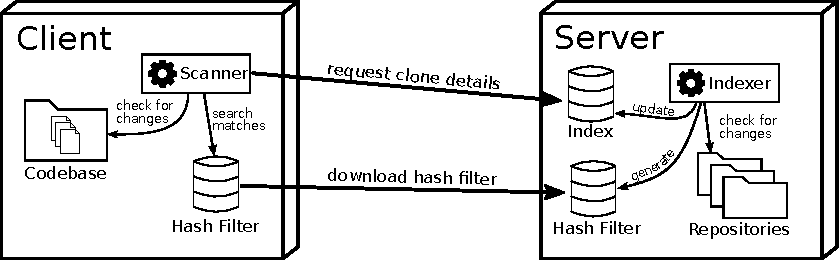
\includegraphics[width=\linewidth]{figures/architecture_overview.pdf}
	\caption{Tool Architecture Overview}\label{fig:tool_architecture}
\end{figure}
\autoref{fig:tool_architecture} shows an overview of the tool's client-server architecture.
The server's purpose is to provide a lookup service for similar code.
The client has a codebase which should be checked for license infringements.
It can use the server's service to find code in its codebase which is similar to code in open source systems.

The server has access to a pool of repositories and creates the index by normalizing and hashing files in those repositories as described in \autoref{section:approach/creating_index/normalization}.
\autoref{section:approach/creating_index/history_analysis} explains how the history of the reference system is analyzed.
Details about the generation of a hash filter are provided in \autoref{section:approach/creating_index/hash_filter}.

The client's search is two staged as described in \autoref{section:approach/searching_copied_code}.
First, the scanner on the client normalizes and hashes code files in its codebase the same way the server does.
During the first stage, the hash filter is used to exclude hashes, which are not part of the server's index.
The hash filter can be downloaded from the server.
The second stage then requests the clone details from the server for the remaining hashes.
This can be done in a continuous manner, i.e. with every change on the client's codebase.

\section{Creating the Index}\label{section:approach/creating_index}
The index is based on the work of Hummel et al. \cite{hummel2010index}.
Source code files are considered as a list of statements.
Sequences of statements of a specific length - so called chunks - are compared by normalizing them, calculating the hash and then comparing the hash values.
Normalizing in this context means reducing the statements to the parts of the code, which describe its structure and increase similarity as described in \autoref{section:approach/creating_index/normalization}.

An index is a data structure which can be used to quickly look up values for a specific key.
For the index, a key-value store is used, which is a database representing a huge key-value map, where a key, e.g. a hash, points to a value.
To add a source code file to the index, first it is parsed and split into tokens.
A token represents a small part of the code such as a symbol, keyword, identifier, literal or comment.
The tokens then are normalized as described in \autoref{section:approach/creating_index/normalization}.
Next, the tokens are aggregated into statements.
The tool then passes over the resulting list of statements using a sliding window to group together a chunk of code, which consists of several consecutive statements.

Chunks are hashed to reduce the space needed to store the information, which is required to identify similar code.
The hashes are then used as the key for the entry in the index.
The value associated with the key of the entry is a list of those locations, where chunks with the hash in question can be found.
A client can then look for similar code by normalizing and calculating the hashes of chunks in the same way, which is detailed in \autoref{section:approach/searching_copied_code}.

The hash of a chunk changes, as soon as the normalized code of that chunk is not exactly the same anymore. 
The amount of statements in a chunk influences the success rate of the algorithm, because longer chunks reduce the probability of finding chunks with modified, added or removed statements.
However, shorter chunks require less statements, which have to be the same to trigger a match.
Therefore, the length of a chunk has to be short enough to find sequences of statements with modifications as shown in \autoref{fig:modification}, but long enough, to exclude generic code, which would produce huge amounts of false positives.

\begin{figure}[h]
	\centering
	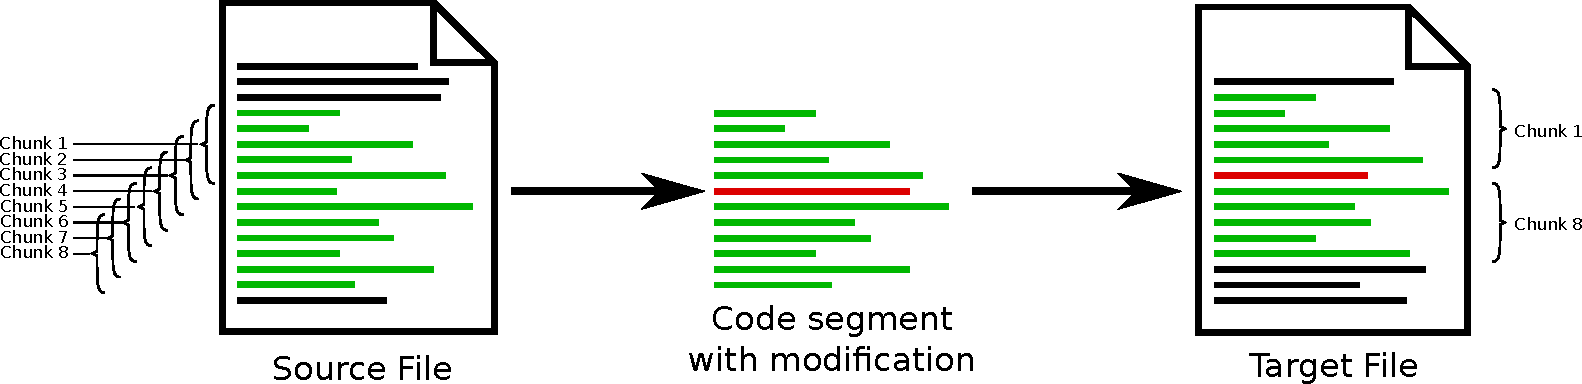
\includegraphics[width=\linewidth]{figures/modification.pdf}
	\caption{Detection of copied code with modification}\label{fig:modification}
\end{figure}

\subsection{Normalization}\label{section:approach/creating_index/normalization}
The normalization step removes irrelevant information and by that brings the features and properties of the code relevant for comparing potentially copied code into focus.
The level of similarity required for a match between two code segments can be adjusted by refining the level of normalization.
The parsing of code into tokens already performs the first part of normalization by removing any formatting.
After that, irrelevant tokens like access modifiers, import or include statements, comments or symbols like brackets or semicolons are removed.
The remaining tokens contain the main information relevant for comparing two sequences of code, since they represent those parts of the code, which is relevant to decide with a high probability, whether it has been copied.

\subsection{History Analysis}\label{section:approach/creating_index/history_analysis}
It is also important to index old versions of the reference system, in order to detect code, which has been copied from older versions of an open source system.
To keep the index up to date and keep information needed to find similarities with older versions of the file, changed files of reference systems are re-indexed.
For that, the server normalizes the new version of the file the same way as described before, groups it into chunks and finally hashes those chunks.
The resulting hashes are then inserted into the key value store.
If an entry for a hash already exists in the index, linking to a file within the same reference project and the same path, the old link is replaced with the new one to save space.
This ensures that the entry for a chunk corresponding to a hash always points to the latest version of a file and that chunks of all versions of a file can still be found in the index.
When files are deleted, nothing is changed in the key-value store to keep the latest existing version of the file's chunk in the key-value store.

Instead of rescanning the whole file, it would be possible to rescan only those chunks which have changed.
However, because the locations of hashes for chunks which did not change also have to be updated in order to keep the latest version of a file in the index, rescanning the file makes sense and simplifies the implementation.

\subsection{Hash Filter}\label{section:approach/creating_index/hash_filter}
It is expected, that most of the calculated hashes of a target system can not be found in the index, since only small portions of code are copied.
Instead of sending a lookup-request for every hash to the server, a better option would be a local copy of the index for faster lookup and less load on the server.
However, the index is very big, because it may contain hashes and the corresponding locations for billions lines of code.
The distribution of such a large index to clients is a challenge, especially as the index has to be updated regularly.

Using a table of all the hashes contained in the index, the client would be able to lookup whether a hash is in the index at all and only has to send a request to the server in this rare case.
This significantly speed up the analysis, since only those hashes which are in the index would be looked up.
Additionally this also reduces the load on the server-side.

Hashing with MD5 reduces the entropy of a chunk to about 128 bit, while still keeping the probability of collisions at a minimum.
Lossless compression is expected to reduce the size of the list of hashes not by much, since the randomness of hashes is very high.
However, lossy compression could be used.
One great way to reduce the size of a list of hashes with a low probability for false positives is a Bloom filter \cite{bloom1970filter}.

To store a value, a Bloom filter uses multiple hash functions to hash a value.
It then uses the resulting hash values as indexes to set bits of a very large bit array to 1.
To determine whether a value is stored in the Bloom filter, the value is hashed with the same hash functions as for storing a value.
Again, hash values are used as indexes.
If all values inside the bit array defined by the indexes are set to 1, the value is part of the index on the server with a very high probability.
If one or more of the bits are set to 0, the value is definitely not in the filter.
For the tool developed in this work, the values inserted into the Bloom filter are the hashes of the chunks.

The advantage is the small size of the filter.
However, there is a certain probability for false positives.
The probability depends on the size of the bit array, the number of inserted values and the number of used hash functions, but when kept at an optimum, grows almost (due to the discrete number of hashing functions) linearly with the number of insertions.
Since it is not possible to remove values from the filter, recalculation is required every time the index changes.

It is also possible to use the filter only to find code in a codebase which has a high probability of being copied.
This may be relevant for proprietary code with high confidentiality.
However, this does not allow the client to further investigate the code section and find the origin for a potential match automatically.
	
\section{Searching Copied Code}\label{section:approach/searching_copied_code}
The client has access to a codebase which should be searched for copied code.
To do so, it normalizes the code in question, groups the resulting statements and hashes them as described in \autoref{section:approach/creating_index}.
After that, the emerging hashes are filtered with the Bloom filter.
The remaining hashes are then sent to the server, which responds with a map of hash to location for each hash.
As explained before, a hash may not be part of the index, but still pass the filter.
This false positive is recognized by the server and excluded from the response.
By aggregating matches by reference system and file path on the client, the relevance of the match can be assessed, as described in \autoref{section:implementation/finding_matches}.
\autoref{fig:search_activity} shows the interaction between client and server.
\begin{figure}[h]
	\centering
	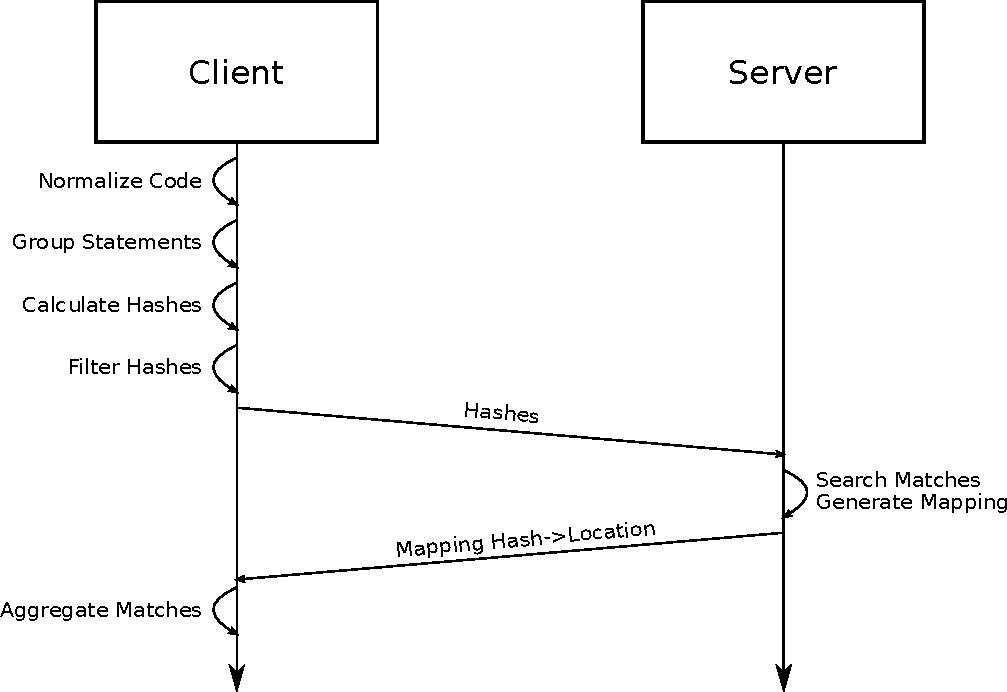
\includegraphics[width=\linewidth]{figures/searching_copied_code.pdf}
	\caption{Visualization of the search process}\label{fig:search_activity}
\end{figure}